% Канонический TikZ-рисунок варианта 01. Править только здесь.
\long\def\figStereoV01{%
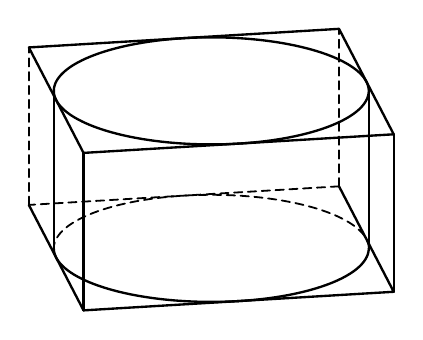
\begin{tikzpicture}[
    x={(1cm,0cm)},
    y={(0cm,0.34cm)},
    z={(0cm,1cm)},
    line cap=round,
    line join=round,
    visible/.style={line width=0.85pt},
    hidden/.style={
        line width=0.65pt,
        dashed,
        dash pattern=on 3pt off 2pt
    }
]

% =========================================================
% Параметры рисунка
% =========================================================

\def\r{2}       % радиус основания цилиндра
\def\H{2}       % высота цилиндра и призмы
\def\phi{10}    % угол поворота квадратного основания

% Радиус описанной окружности квадрата
\pgfmathsetmacro{\R}{sqrt(2)*\r}

% =========================================================
% Вершины нижнего основания призмы
% =========================================================

\coordinate (A0) at
    ({\R*cos(45+\phi)},{\R*sin(45+\phi)},0);

\coordinate (A1) at
    ({\R*cos(135+\phi)},{\R*sin(135+\phi)},0);

\coordinate (A2) at
    ({\R*cos(225+\phi)},{\R*sin(225+\phi)},0);

\coordinate (A3) at
    ({\R*cos(315+\phi)},{\R*sin(315+\phi)},0);

% =========================================================
% Вершины верхнего основания призмы
% =========================================================

\coordinate (B0) at
    ({\R*cos(45+\phi)},{\R*sin(45+\phi)},\H);

\coordinate (B1) at
    ({\R*cos(135+\phi)},{\R*sin(135+\phi)},\H);

\coordinate (B2) at
    ({\R*cos(225+\phi)},{\R*sin(225+\phi)},\H);

\coordinate (B3) at
    ({\R*cos(315+\phi)},{\R*sin(315+\phi)},\H);

% =========================================================
% Невидимое заднее ребро нижнего основания
% =========================================================

\draw[hidden] (A0)--(A1);

% =========================================================
% Невидимые вертикальные рёбра
% =========================================================

\draw[hidden] (A0)--(B0);
\draw[hidden] (A1)--(B1);

% =========================================================
% Невидимая часть нижней окружности цилиндра
% =========================================================

\draw[hidden]
    plot[
        domain=0:180,
        samples=100,
        variable=\t
    ]
    ({\r*cos(\t)},{\r*sin(\t)},0);



% =========================================================
% Видимые рёбра нижнего основания
% =========================================================

\draw[visible] (A1)--(A2)--(A3)--(A0);

% =========================================================
% Видимые вертикальные рёбра призмы
% =========================================================

\draw[visible] (A2)--(B2);
\draw[visible] (A3)--(B3);

% =========================================================
% Образующие цилиндра
% =========================================================

\draw[visible] (-\r,0,0)--(-\r,0,\H);
\draw[visible] ( \r,0,0)--( \r,0,\H);

% =========================================================
% Видимая часть нижней окружности цилиндра
% =========================================================

\draw[visible]
    plot[
        domain=180:360,
        samples=100,
        variable=\t
    ]
    ({\r*cos(\t)},{\r*sin(\t)},0);

% =========================================================
% Верхнее основание призмы
% =========================================================

\draw[visible]
    (B0)--(B1)--(B2)--(B3)--cycle;

% =========================================================
% Верхнее основание цилиндра
% =========================================================

\draw[visible]
    plot[
        domain=0:360,
        samples=160,
        variable=\t
    ]
    ({\r*cos(\t)},{\r*sin(\t)},\H);

\end{tikzpicture}
}
